\documentclass[11pt]{article}
\usepackage[T1]{fontenc}      % proper glyphs (<, >, |) and hyphenation
\usepackage{lmodern}
\usepackage{amsmath}
\usepackage[margin=1in]{geometry}
\usepackage{graphicx}\graphicspath{{figures/}}
\usepackage{booktabs}
\usepackage{tabularx}
\usepackage{microtype}
\usepackage{xcolor}
\usepackage{hyperref}
\usepackage{xurl}              % break long URLs at safe characters
\usepackage[htt]{hyphenat}    % allow breaks inside \texttt{} (file paths)
% Float budget: a short document with many floats otherwise strands them after the last section.
\renewcommand{\topfraction}{0.9}
\renewcommand{\bottomfraction}{0.7}
\renewcommand{\textfraction}{0.1}
\renewcommand{\floatpagefraction}{0.75}
\sloppy                        % prefer loose spacing over right-margin overflow
\emergencystretch=3em          % last-resort stretch for unbreakable lines
% PPI theme -- Progress and Poverty Institute brand styling.
% Colors sampled from progressandpovertyinstitute.org (indigo family + coral accent).
% Requires xcolor (loaded in the main preamble) and hyperref.
\definecolor{ppiprimary}{HTML}{475BB2}  % indigo (primary brand)
\definecolor{ppidark}{HTML}{2D3559}     % deep navy
\definecolor{ppilight}{HTML}{579AF6}    % sky accent
\definecolor{ppiaccent}{HTML}{FF4F55}   % coral accent
\usepackage{sectsty}
\allsectionsfont{\color{ppidark}}
\hypersetup{colorlinks=true,linkcolor=ppiprimary,urlcolor=ppiprimary,citecolor=ppiprimary}


% Generated headline numbers — produced by paper/scripts/generate_paper_assets.py.
% Run that generator BEFORE writing/compiling prose; never type result numbers here.
\InputIfFileExists{tables/headlines.tex}{}{}

\begin{document}

\begin{center}
  \IfFileExists{figures/ppi-logo.pdf}{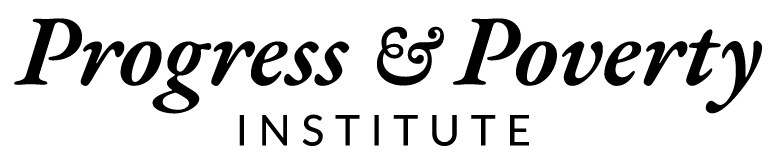
\includegraphics[height=1.3cm]{ppi-logo}\\[0.6em]}{\IfFileExists{figures/ppi-logo.png}{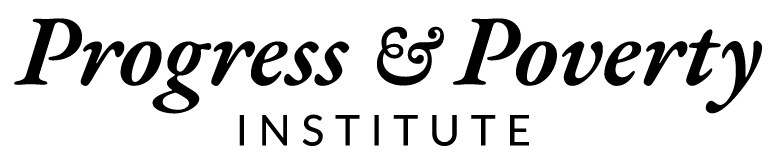
\includegraphics[height=1.3cm]{ppi-logo}\\[0.6em]}{}}{\LARGE\bfseries\color{ppiprimary} Fixing Philadelphia's land assessments without moving anyone's total\par}
  \vspace{0.35em}
  {\large\color{ppidark} What a zone-rate land allocation would do to tax bills, and how it measures against the draft land-assessment ordinance\par}
  \vspace{0.7em}
  {\large Russell Richie\par}
  \vspace{0.2em}
  {\normalsize Progress and Poverty Institute\par}
  \vspace{0.2em}
  {\normalsize \today\par}
\end{center}
\vspace{1em}

\begin{abstract}
\noindent A draft ordinance before Philadelphia City Council would, for the first time, tell
the Office of Property Assessment what the land half of an assessment has to mean --- the
market value of the lot as if vacant --- and forbid the shortcut OPA uses today, which is to
call land a fixed fifth of whatever the whole property is worth. This report asks what the
smallest change that satisfies the ordinance's purpose would do to tax bills, using the
simplest candidate: keep the fixed fraction, but apply it to a market-area rate per square
foot instead of to each parcel's own total (the ``LYCD'' allocation). Two readings of that
proposal give opposite answers. Read as a \emph{revaluation}, with land re-valued and the
building left alone, it moves every bill in the city and cuts \LycdADownTenPct{} of them by
more than a tenth --- but two-thirds of the increases land on vacant lots, where the method's
land values run \LycdSalesLYCDAgg{} what those lots actually sell for, and the sum of land and
building exceeds the parcel's own assessment on \LycdAOvershootPct{} of improved parcels. Read
as the ordinance is written --- a re-split \emph{inside} each parcel's unchanged total, with
the tax rate untouched --- it moves \LycdCMoved{} bills (\LycdCMovedPct{}), every one of them a
parcel with a construction abatement, and lowers the levy by \LycdCLevyAbsM{} (\LycdCLevyPct{}),
because OPA today assesses abated lots at \LycdUniOPAAbatedRatio{} their neighbours'. On the
ordinance's own uniformity tests the two methods fail different clauses: OPA's land component
is a deterministic function of the building on it (rank correlation \LycdUniOPABuildingCorr{}
across \LycdUniCells{} zone-and-lot-size cells), while the raw allocation gives a vacant lot
\LycdUniLYCDVacantImprovedRatio{} the land rate of the identical improved lot beside it. The
re-split inherits the better half of each. What it cannot do is make land values \emph{accurate}
on the one class where accuracy can be checked against sales, and the ordinance's accuracy
report would say so in its first year. A second analysis asks whether anything can. Built from
\LycdWitN{} land sales --- bare lots, lots sold bare and since built on, and teardowns --- and
scored held-out, a paired-sales comparables surface (each parcel's land rate the adjusted
median of its ten nearest land sales) is less dispersed than OPA's land values by
\LycdSfiveVsSzeroDiffAbs{} COD and than a published rate schedule built from the same sales by
\LycdSfiveVsSthreeDiffAbs{}; the schedule is indistinguishable from OPA. Swapped into the same
tax model, it reverses the sign of the ordinance's fiscal effect --- the levy
\LycdSfiveCLevySign{} by \LycdSfiveCLevyAbsM{} rather than falling --- so the direction depends on
the land model, and the one the sales support goes the other way. The land model also decides
who a land tax would fall on. A 4:1 split-rate built on OPA's land values or on the allocation is
flat to regressive by neighbourhood income and race. Built on the sales-based surface it is
progressive on both: homes' total bill changes by \LycdEqSfiveEndsHomesNonwhite{} in the most
non-white fifth of block groups against \LycdEqSfiveEndsHomesWhite{} in the whitest, and by
\LycdEqSfiveEndsHomesPoor{} in the poorest fifth against \LycdEqSfiveEndsHomesRich{} in the
richest. That ordering holds under every treatment of the construction abatement.
\end{abstract}

\section{The question}

Section 2-305 of the Philadelphia Code already requires OPA to publish a methodology and an % noqa: hardcode
annual assessment-sales ratio study, and to submit to an independent audit every three years.
None of those provisions says anything about the land component of an assessment. OPA
publishes a land value and an improvement value for every parcel, and nothing in the Code says
what the land value must represent or requires anyone to test whether it does. The draft
ordinance now circulating in discussion form would close that gap in three moves: a standard
(the land component ``shall closely approximate the market value of the land as if vacant''
and ``shall not vary among similarly situated parcels on the basis of the presence, absence,
condition, or value of improvements''); a prohibition (it ``shall not be determined by the
application of a fixed percentage or ratio to total assessed value''); and a test (a separate
annual land value accuracy report, with the same statistical standards the total already faces).

The prohibition is aimed at a specific practice. In the TY\LycdTaxYear{} roll,
\LycdDefaultRatioOpaPct{} of the city's \LycdDefaultRatioImprovedParcels{} improved parcels carry a
land component that is exactly \LycdDefaultRatioOpaMode{} of their total assessment
(Figure~\ref{fig:defaultratio}). That is not a market finding; it is a rule of thumb. It has a
consequence the ordinance's findings name directly --- it ``distort[s] the taxable base of
properties receiving partial exemptions or abatements'' --- and a consequence they do not name,
which matters more for anything Council might later want to do with land values: a land
component that is a fixed share of total value is, by construction, a function of the building.
Two identical lots on the same block get different land values if one has a nicer house on it.

The live question is what to replace the rule of thumb with. The ordinance's answer is the
full appraisal toolkit --- vacant sales, teardown sales, extraction from improved sales, paired
sales, location value surfaces --- and an interim certification for any class where the
evidence is too thin. That is the right long-run answer. But it is a multi-year build for an
office that has never modeled land, and there is a much smaller change available in the
meantime: keep the fixed fraction, and stop applying it to the parcel's own total. Apply it
instead to a rate per square foot estimated for the parcel's market area, and multiply by the
lot. The land value then depends on where the lot is and how big it is, and on nothing else.
That is the construction this report tests, under the name it carries in the modeling
literature, LYCD.\footnote{``Least You Can Do'' (Lars Doucet). For an improved parcel,
$\text{land} = \LycdLycdKImproved{} \times \text{median}(\text{total value}/\text{lot area})_{\text{zone}} \times \text{lot area}$,
with the zone taken from OPA's own Geographic Market Area hierarchy. For a vacant parcel the
multiplier is \LycdLycdKVacant{}. Land is capped at the parcel's own total. The construction,
its defects, and the path from it to an assessor-grade land model are documented in
\texttt{docs/LYCD\_LAND\_MODEL\_ROADMAP.md} in the LVTShift repository.}

Two things follow that a reader should hold onto. First, this proposal would fall inside the
ordinance's prohibition as drafted --- it is a fixed percentage applied to total value, one
step removed --- so adopting it means amending the prohibition, and Section~\ref{sec:language}
offers language. Second, ``use it to value land'' can mean two different reforms, and they
have opposite effects on bills. The next section separates them.

\section{Two reforms wearing one name}\label{sec:readings}

Suppose OPA replaced its land component with the zone-rate allocation and left the tax rate
alone. What happens to a bill depends entirely on what happens to the \emph{building}
component, and there are two defensible answers.

\begin{enumerate}
\item \textbf{Revaluation.} The new land value is added to OPA's existing building value. The
  parcel's total assessment changes --- upward, for most parcels, since the allocation puts more
  value in land than OPA's fifth does. Every bill in the city moves. If the rate is then rolled
  back so the levy is unchanged (reading A), the question is who wins and who loses; if it is
  not (reading B), the levy simply rises.
\item \textbf{Re-split.} The parcel's total assessment is held where OPA put it, and the new
  land value is carved out of it; the building component becomes the remainder. This is what
  the ordinance describes. Its Section~3(c) makes land and improvement ``complementary parts of
  a single assessment at actual value,'' and its findings assert that the change ``does not
  alter the total assessed value of any parcel, the applicable tax rate, or the tax liability of
  any property that is not subject to a partial exemption or abatement.'' With the total and the
  rate both fixed, a bill can only move if some exemption depends on how the total is split.
  The Homestead Exemption does not --- it is a flat amount off the total. The ten-year
  construction abatement does --- it exempts the assessed value of the \emph{improvement}. So
  only abated and partially-exempt parcels can move (reading C).
\end{enumerate}

\begin{table}[t]
  \centering
  \caption{Three readings of ``LYCD land, rates unchanged.'' Only the third is the reform the
  ordinance describes. Bills counted over the \LycdBilledParcels{} parcels with a nonzero bill
  today.}
  \label{tab:scenarios}
  \input{tables/scenarios.tex}
\end{table}

Table~\ref{tab:scenarios} puts the three side by side. The revaluation readings move
\LycdBilledParcels{} bills; the re-split moves \LycdCMoved{}. That difference is not a
modeling choice. It is the difference between a reform that changes what properties are worth
and a reform that changes what the two lines on an assessment notice mean. The ordinance is
the second kind, and the rest of this report treats the re-split as the primary result and
the revaluation as the contrast that shows what is \emph{not} being proposed.

\section{Data and method}

Every parcel figure comes from OPA's certified TY\LycdTaxYear{} roll (\LycdParcels{} parcels;
\LycdBilledParcels{} with a nonzero bill after the Homestead Exemption, abatements and
institutional exemptions), at the year's combined City and School District rate of
\LycdMillage{} mills. The zone-rate land allocation is computed exactly as the LVTShift
repository's four Philadelphia land-tax models compute it, from one shared function, and is
checked against the tracked export of those models on every run.

\paragraph{Carrying exemptions through a changed split.} Both readings need every existing
exemption re-applied to a parcel whose land component has moved. The rule: the Homestead
Exemption is re-applied as the statutory amount or the total, whichever is smaller, against
the building line first; an abatement is a share of the building line (the abated dollars
divided by the building) and is re-applied as that share of the new building component; partial
institutional relief that reaches the land line is a share of total value and is carried in
dollars; a parcel that is fully exempt for a reason the homestead cannot explain stays fully
exempt. The rule is validated by reconstruction: feeding OPA's own land back through it must
reproduce OPA's own taxable value parcel by parcel, and it does so on \LycdReconMatchPct{} of the roll. The
remaining half-percent are parcels where OPA's recorded homestead flag disagrees with the
relief actually applied; the re-split's effect is measured against the rule's own
reconstruction rather than against the recorded bill, so that residual cancels instead of
appearing as a tax change.\footnote{This mattered. Measured against recorded bills, the
re-split appeared to move about two thousand additional parcels whose exemption does not
depend on the split at all. Every parcel the re-split moves is asserted, on every run, to carry
abatement-type relief.}

\paragraph{The ordinance's tests.} Section~3(b)'s uniformity standard and Section~4(c)'s
required tests are operationalized within OPA's own finest market geography (the L3 Geographic
Market Area), comparing land value per square foot for vacant against improved parcels, for
abated against unabated parcels, and --- the sharpest form --- rank-correlating land value with
building value among improved parcels in the same zone and the same lot-size quartile. Its
accuracy standard is tested the only way it can be for a land value: against sales of bare
lots, where the sale price is the land price. That study uses \LycdSalesN{} vacant sales since
2023, filtered to plausible lot sizes and prices and to parcels with no building footprint.

\section{What the ordinance's reform does to bills}\label{sec:resplit}

\begin{table}[t]
  \centering
  \caption{The re-split, by kind of exemption. With the total and the rate held fixed, only an
  exemption that depends on the land/building split can change a bill. Net change at the
  unchanged rate of \LycdMillage{} mills.}
  \label{tab:fiscal}
  \input{tables/fiscal_note.tex}
\end{table}

\LycdCUnchangedParcels{} of \LycdBilledParcels{} bills --- \LycdCUnmovedPct{} --- do not change by
a cent. Table~\ref{tab:fiscal} shows why: no parcel without an exemption moves, no parcel with
only a homestead moves, and no parcel with partial relief on its total value moves. The
\LycdCMoved{} that do move all carry abatement-type relief, and the levy falls by \LycdCLevyAbsM{}
(\LycdCLevyPct{}), which is the fiscal note the ordinance's drafting notes ask for. The direction
is the interesting part. The drafters flagged it as unknown --- ``a fiscal note should model
both directions'' --- and on this construction it is negative: \LycdCDown{} abated bills fall and
\LycdCUp{} rise, \LycdCDownM{} against \LycdCUpM{}.

\begin{table}[t]
  \centering
  \caption{Where the re-split lands. Parcels whose bill moves, by property type; the last
  column is the median ratio of the new land component to OPA's, over those parcels.}
  \label{tab:movers}
  \input{tables/movers_category.tex}
\end{table}

Why negative? Because OPA's fifth-of-total rule, applied to a new building, produces a land
value that has nothing to do with the lot. A new house assessed at several times its
neighbours' gets a land component several times theirs, on an identical lot, and
\LycdAbatedAtDefaultPct{} of abated parcels sit at exactly the default ratio. Within a market
area, OPA assesses abated parcels' land at \LycdUniOPAAbatedRatio{} the rate of unabated
parcels'; the zone-rate allocation assesses it at \LycdUniLYCDAbatedRatio{}, by construction. So
when the re-split replaces OPA's inflated land component with the zone rate, an abated parcel's
taxable value --- which under a full abatement is its land component --- falls. The category
that is nothing but full ten-year abatements (Table~\ref{tab:movers}) sees a median cut of
\LycdCAbatedMedianAbsPct{}, on a land component now \LycdCAbatedLandRatio{} what OPA had, and it
accounts for \LycdCAbatedShareOfNet{} of the net change. The \LycdCSfrMoved{} single-family
homes that move carry partial abatements and move by a median of \LycdCSfrMedianAbs{}, nine in
ten by less than \LycdCSfrNinetiethAbs{}. Figure~\ref{fig:maps} (right) shows the geography: the
reductions concentrate where the new construction is, in and around Center City, and the rest
of the map is white.

\begin{figure}[t]
  \centering
  \includegraphics[width=\linewidth]{scenario_maps.pdf}
  \caption{Left: the revaluation (reading A), median change in bill by Census tract, clipped
  at $\pm$\LycdMapPctClip\%. Right: the re-split (reading C), net change in tract bills in
  thousands of dollars. Tracts with no billed parcels are omitted.}
  \label{fig:maps}
\end{figure}

This is the finding to carry into the fiscal note. It is not that abatements get bigger. It is
that OPA has been assessing abated parcels' land at nearly double the going rate for their
block, because the rule of thumb scales land with the building, and a land standard that stops
that will --- on this construction --- lower those bills. Whether the zone rate is the
\emph{right} land value for a lot that was recently bought and built on is a fair question, and
Section~\ref{sec:standards} returns to it. But the current premium is not evidence about those
lots. It is arithmetic.

\section{What a revaluation would do instead}\label{sec:reval}

The revaluation readings are worth reporting because they are what a reader who hears ``LYCD
land values'' is likely to imagine, and because the contrast is sharp.

\begin{table}[t]
  \centering
  \caption{The revaluation (reading A), by property type. Land re-valued by the zone-rate
  allocation, OPA's building value kept, rate rolled back from \LycdMillage{} to
  \LycdAMillage{} mills to hold the levy.}
  \label{tab:reval}
  \input{tables/revaluation_category.tex}
\end{table}

Adding the zone-rate land value to OPA's building value raises the taxable base enough that the
rate can fall \LycdAMillageCutAbsPct{}, to \LycdAMillage{} mills, and still raise the same
\LycdLevyB{}. At that rate \LycdADownTenPct{} of bills fall by more than ten percent and
\LycdAUpTenPct{} rise by more than ten percent; the median single-family bill falls
\LycdASfrMedianAbsPct{} (Table~\ref{tab:reval}). Left unrolled (reading B), the levy would rise
\LycdBLevyRisePct{} to \LycdBLevyB{}. Stratified by neighbourhood income and racial composition,
the revaluation is close to flat --- between \LycdAEquityQOneWin{} and \LycdAEquityQFiveWin{} of
parcels pay less in every income quintile, with overlapping intervals across racial-composition
bands (Table~\ref{tab:equity}) --- with one exception: in the lowest decile of property value
only \LycdAEquityDOneWin{} pay less and the median bill rises \LycdAEquityDOneMedian{}. That
decile is where the vacant lots are.

\begin{table}[t]
  \centering
  \caption{The revaluation (reading A) by block-group income quintile and racial composition.
  Winners are parcels whose bill falls; intervals are bootstrap 95\% bands.} % noqa: hardcode
  \label{tab:equity}
  \input{tables/equity.tex}
\end{table}

\begin{figure}[t]
  \centering
  \includegraphics[width=\linewidth]{scenario_compare.pdf}
  \caption{Distribution of the change in the annual bill under the two readings, log scale,
  clipped at $\pm$\LycdScenarioHistClip\%. The revaluation moves everything; the re-split
  leaves \LycdCUnmovedPct{} of bills at zero.}
  \label{fig:compare}
\end{figure}

Two facts keep this from being a headline. First, the money moving toward vacant land is the
method's best-documented error, not a finding. Vacant lots' bills rise by a median
\LycdAVacantMedianPct{} and account for \LycdAVacantShareOfShift{} of all the dollars that
increase, and the sales test in Section~\ref{sec:standards} shows the allocation values bare
land at \LycdSalesLYCDAgg{} its sale price in aggregate. Roughly, the revaluation moves
\LycdAVacantNetM{} onto vacant land, and the sales evidence says something like half of that is
a mistake. Second, the revaluation breaks the identity the ordinance is built on. Adding a new
land value to an old building value means land plus building exceeds the parcel's own
assessment on \LycdAOvershootParcels{} of \LycdAOvershootDenom{} improved parcels
(\LycdAOvershootPct{}), by \LycdAOvershootB{} in aggregate. Under Section~3(c) that is not a
permitted assessment. The revaluation is a useful model of a land-tax \emph{distribution}; it is
not a model of this ordinance, and it should not be read as one.

\section{The zone-rate allocation against the ordinance's standards}\label{sec:standards}

The ordinance sets two standards for the land component and requires an annual report against
both. The report OPA would have to publish in its first year, applied to the two candidate land
surfaces, would say the following.

\subsection{Section 3(e): the prohibited practice}

\begin{figure}[t]
  \centering
  \includegraphics[width=0.9\linewidth]{default_ratio.pdf}
  \caption{Land as a share of total assessed value, improved parcels, log scale, clipped at
  \LycdRatioHistClip{}. OPA's roll piles up at \LycdDefaultRatioOpaMode{}; the zone-rate
  allocation, re-split inside the same totals, spreads.}
  \label{fig:defaultratio}
\end{figure}

Figure~\ref{fig:defaultratio} is the practice the ordinance prohibits, seen directly.
\LycdDefaultRatioOpaPct{} of improved parcels sit at the default ratio in OPA's roll;
\LycdDefaultRatioLycdPct{} do after the re-split. The zone-rate allocation is also a fixed
percentage --- but of a market-area rate, not of the parcel's own value, and the difference is
exactly what makes the next test come out differently.

\subsection{Section 3(b), second sentence: uniformity across improvements}

\begin{table}[t]
  \centering
  \caption{The ordinance's uniformity tests within OPA's L3 market areas. Rows 1 and 2 are the
  median, over zones, of the ratio of median land \$/sqft between the two groups; row 3 is the
  median Spearman correlation over zone-and-lot-size-quartile cells with at least thirty
  parcels. ``LYCD, raw'' is the allocation as the method publishes it; ``LYCD, re-split'' is
  what the ordinance would certify, with each parcel's land capped at its own total.}
  \label{tab:uniformity}
  {\small\input{tables/uniformity.tex}}
\end{table}

Table~\ref{tab:uniformity} is the center of this report. The ordinance says the land
component ``shall not vary among similarly situated parcels on the basis of the presence,
absence, condition, or value of improvements.'' Both surfaces fail that sentence, and they fail
different halves of it.

OPA fails on \emph{value}. Among improved parcels in the same market area and the same
lot-size quartile --- as close to ``similarly situated'' as this data can get --- the rank
correlation between OPA's land component and the value of the building on it is
\LycdUniOPABuildingCorr{}, across \LycdUniCells{} such cells. That is not a strong association;
it is a function. Land equals a fifth of total, total equals land plus building, so land equals
a quarter of the building, and a more valuable house on the same size lot on the same block gets
a more valuable lot. It is also, as the previous section showed, why abated parcels' land runs
\LycdUniOPAAbatedRatio{} their neighbours'. The zone-rate allocation cuts the correlation to
\LycdUniLYCDBuildingCorr{} and the abatement premium to \LycdUniLYCDAbatedRatio{}.

The raw allocation fails on \emph{presence}. Its vacant multiplier is \LycdLycdKVacant{} and its
improved multiplier is \LycdLycdKImproved{}, so within every one of
\LycdUniLYCDVacantImprovedZones{} market areas a vacant lot is assigned \LycdUniLYCDVacantImprovedRatio{}
the land rate of the improved lot beside it (Figure~\ref{fig:uniformity}). That is variation on
the basis of the absence of improvements, in the exact words of the standard, and OPA does not
have it: its vacant and improved land rates agree at the zone median
(\LycdUniOPAVacantImprovedRatio{}).

\begin{figure}[t]
  \centering
  \includegraphics[width=\linewidth]{uniformity.pdf}
  \caption{Land value per square foot for vacant and improved parcels, all L3 market areas
  pooled, log scale, top percentile trimmed. OPA's two distributions sit on top of each other;
  the raw allocation's do not, because its vacant leg uses a multiplier of \LycdLycdKVacant{}
  where its improved leg uses \LycdLycdKImproved{}.}
  \label{fig:uniformity}
\end{figure}

But the re-split does not publish the raw allocation. It caps each parcel's land at its own
total, and a vacant parcel's total \emph{is} its land, so under the ordinance's reform every
vacant lot keeps OPA's own vacant value. The certified surface therefore inherits OPA's
vacant--improved agreement (\LycdUniResplitVacantImprovedRatio{}) and the allocation's
building-independence (\LycdUniResplitBuildingCorr{}, \LycdUniResplitAbatedRatio{} on abated
lots). On the uniformity sentence, the re-split is the best of the three columns. That is a
real result, and it is the strongest case for the minimal change.

\subsection{Section 3(b), first sentence, and Section 4(b): accuracy}

\begin{table}[t]
  \centering
  \caption{Assessed land value divided by sale price, vacant-land sales since 2023, both
  surfaces. A ratio of 1.00 is right. The IAAO standard for the coefficient of dispersion % noqa: hardcode
  is \LycdIaaoCod{}.}
  \label{tab:sales}
  {\small\input{tables/vacant_ratio.tex}}
\end{table}

The first sentence of the standard is that the land component ``shall closely approximate the
market value of the land as if vacant,'' and Section~4(b)(.1) names the test: compare it to
sales of vacant land. Table~\ref{tab:sales} and Figure~\ref{fig:sales} apply that test to both
surfaces on \LycdSalesN{} bare-lot sales. Neither passes. OPA assesses bare land at
\LycdSalesOPAAgg{} its sale price in aggregate (median \LycdSalesOPAMedian{}); the raw
allocation, at \LycdSalesLYCDAgg{} (median \LycdSalesLYCDMedian{}). Both are dispersed far beyond
the IAAO limit --- coefficients of dispersion of \LycdSalesOPACod{} and \LycdSalesLYCDCod{}
against a standard of \LycdIaaoCod{} --- and both are regressive, with price-related
differentials of \LycdSalesOPAPrd{} and \LycdSalesLYCDPrd{} where uniformity wants about one:
cheap lots over-assessed, expensive lots under-assessed, on both surfaces.

\begin{figure}[t]
  \centering
  \includegraphics[width=\linewidth]{sales_test.pdf}
  \caption{The Section~4(b)(.1) test. Left: aggregate assessed-to-sale ratio, where the dashed
  line is correct. Right: coefficient of dispersion, where the dashed line is the IAAO limit.
  Three sample cuts of the same sales, narrowing from the left.}
  \label{fig:sales}
\end{figure}

For the minimal change this has a specific meaning. Because the re-split keeps OPA's vacant
values, the certified surface's vacant-land accuracy is OPA's: \LycdSalesOPAAgg{}. The zone-rate
allocation cannot improve it, and the annual accuracy report would say so. What the sales
\emph{can} do is calibrate the method. The allocation's vacant leg is linear in its multiplier,
so a surface running \LycdSalesLYCDAgg{} in aggregate is consistent with a multiplier of
\LycdSalesImpliedKAgg{} rather than \LycdLycdKVacant{} (\LycdSalesImpliedKMedian{} on the
median). That number is worth more than it looks. It is the first sales-based estimate of what
fraction of a market area's total-value rate is land, and it says the answer is a good deal
more than a fifth --- which is also the first piece of evidence about whether the improved
multiplier of \LycdLycdKImproved{} is right. It is not proof: a vacant lot and a built one in the
same zone are not the same lot, and the dispersion behind that aggregate is large. But it is
what the ordinance's Section~4(d) asks for when direct evidence is thin --- an evaluation with
its basis stated --- and it is the natural first entry in OPA's first land value accuracy report.
Section~\ref{sec:sales} goes further and builds the surface those sales support.

\subsection{Section 3(c): the identity}

The re-split satisfies Section~3(c) by construction; land plus building equals OPA's total on
every parcel, to the cent, and the modeling asserts it. The revaluation does not
(Section~\ref{sec:reval}). Any proposal that ``adds'' a land value to OPA's building is outside
the ordinance whatever land value it uses.

\section{A land surface built from the sales}\label{sec:sales}

The zone-rate allocation is the least you can do. The question it leaves open is whether
doing more --- building the land component from land sales, as the ordinance's Section~3(d)
contemplates --- produces something measurably closer to ``the market value of the land as if
vacant,'' and if so in what form. This section reports a second analysis, built in the
sibling \texttt{philly\_open\_avmkit} repository and scored there against the sales, then
swapped into the tax model above.\footnote{\texttt{notebooks/pipeline/run\_land\_surfaces.py};
its generated comparison is \texttt{out/land/report.md}. LVTShift consumes the per-parcel rate
through \texttt{paint\_land\_surface} and re-runs \texttt{model\_lycd\_reassessment.ipynb} with
\texttt{LVT\_LAND\_SURFACE=s5}, so every tax-side figure for the new surface comes through
exactly the code path the LYCD figures did.}

\subsection{The evidence, and what was missing from it}

\begin{table}[t]
  \centering
  \caption{Three streams of land-price evidence, time-adjusted to the valuation date and
  filtered identically (single-parcel deeds, no building footprint on a recorded-vacant lot,
  plausible \$/sqft, no condominium units).}
  \label{tab:witnesses}
  \input{tables/witness_streams.tex}
\end{table}

Every sales test so far --- Section~\ref{sec:standards}'s included --- used lots that are
vacant \emph{today}, because that is the only sample OPA's category code can give you. It is
the wrong sample for the question. The pipeline's ``vacant sale'' flag is current status joined
at download, not status at the time of sale, so a lot that sold bare and has since been built
on is invisible to every vacant-land model. Recovering those sales from the building's
construction year, and adding teardowns (an improved parcel bought and demolished within a
year, identified from completed L\&I demolition permits), gives three streams under one set of
filters (Table~\ref{tab:witnesses}). They disagree by a factor of \LycdWtwoOverWone{}, and they
disagree in a direction that matters. Land nobody built on sells for \LycdWonePsf{} a square
foot at the median; land somebody bought to build on, \LycdWonebPsf{}; land somebody bought
to clear, \LycdWtwoPsf{}. The second and third are independent evidence --- different sales,
different signals --- and both sit far above the first. A surface fitted only to still-vacant
sales is fitted to the land nobody wanted, and \LycdImprovedSharePct{} of the roll is parcels
somebody did.

\subsection{Turning sales into a land value}

\begin{table}[t]
  \centering
  \caption{Held-out accuracy against \LycdHeldoutN{} land sales, all three streams pooled.
  Five folds assigned by parcel; every fitted surface is refitted inside each fold, and the
  extraction is re-levelled inside each fold rather than against the sales it is scored on. The
  COD is trimmed of the outer 5\% of ratios at each end and applied identically to every % noqa: hardcode
  surface; the raw figure is the same statistic untrimmed. \LycdHeldoutUntabulated{} further
  candidates, mostly variants of these, were scored on the same rows and are not shown.}
  \label{tab:heldout}
  \input{tables/heldout.tex}
\end{table}

The ordinance's Section~3(d) lists the recognized ways to get from sales to a land value, and
the second analysis built most of them from the same witnesses: a published rate schedule (a
weighted median rate per OPA market area, cascading to coarser areas where evidence is thin,
with fitted lot-size and sub-minimum-lot adjustments --- the form Section~\ref{sec:language}
argues an assessor could publish); extraction from improved sales; a hierarchical Bayesian model
that estimates land and improved-property values jointly; an interpolation that averages the
nearest sales; openavmkit's modelling engines; and a comparable-sales approach with its
adjustments derived from paired sales. That last one takes each parcel's ten nearest land
sales, adjusts each sale's rate to the parcel's own lot size and sub-minimum status by amounts
measured on pairs of nearby sales that differ in only that attribute, and reconciles by a
weighted median. Table~\ref{tab:heldout} scores the main candidates against the sales they were
not fitted to, alongside the two surfaces that never saw the sales at all.

\begin{table}[t]
  \centering
  \caption{Head to head. Every surface predicts the same held-out rows, so the comparison is
  paired and the rows' shared difficulty cancels; the interval is a bootstrap over parcels. A
  negative difference means the first surface is the less dispersed.}
  \label{tab:h2h}
  \input{tables/head_to_head.tex}
\end{table}

Two results stand out. First, the schedule does not beat the assessor. Against OPA's land
values it is \LycdSthreeVsSzeroDiff{} COD, an interval that straddles zero
(Table~\ref{tab:h2h}), so the published-schedule form costs accuracy against the comparables and the
interpolation and buys nothing OPA does not already have. Second, the paired-sales
surface does beat it. Its trimmed COD is \LycdSfiveTrCod{}, against \LycdSzeroTrCod{} for OPA and
\LycdSthreeTrCod{} for the schedule; paired, it is \LycdSfiveVsSzeroDiffAbs{} COD less dispersed
than OPA and \LycdSfiveVsSthreeDiffAbs{} less than the schedule, with intervals that exclude
zero. The simple interpolation is statistically indistinguishable from it
(\LycdSfiveVsStwoDiff{}, \LycdSfiveVsStwoLo{} to \LycdSfiveVsStwoHi{}), and the Bayesian model
is measurably worse (\LycdSeightVsSfiveDiff{}). The zone-rate allocation is
\LycdSzeroVsSoneDiffAbs{} COD worse than OPA.

Extraction deserves its own sentence, because it is the method an appraiser would reach for
first, and the ordinance names it. Rebuilt without its published calibration --- which
re-levels it against the same vacant sales this study scores on, so as published its accuracy
is in-sample and cannot be compared with anything --- it scores \LycdSfourcvTrCod{}, worse than
OPA's \LycdSzeroTrCod{} by \LycdSfourcvVsSzeroDiffAbs{} COD. It carries real land signal --- its
median ratio is \LycdSfourcvTrMedian{}, so it is not mis-levelled --- but the residual of an
improved sale is a noisier instrument than a land sale, and Philadelphia has enough land sales to
prefer them.

One candidate is more accurate than the paired-sales surface, and it is not the one this report
carries forward. Gradient-boosted trees fitted to the same witnesses score \LycdEgbmTrCod{},
\LycdEgbmVsSfiveDiffAbs{} COD better than paired sales (\LycdEgbmVsSfiveLo{} to
\LycdEgbmVsSfiveHi{}). The land roll the second analysis builds selects the least dispersed
surface among those that pass the improvement-neutrality test below at \LycdTOneBar{} or better,
and holds the boosted trees out for a reason that is not a test result. Their value for a parcel
decomposes into a base rate and factors for location, lot size, sub-minimum status and zoning,
but the location factor is a learned function of coordinates with no sale behind it, so an
owner cannot contest it the way a list of comparable sales can be contested. Whether that meets
the ordinance's explainability and publication requirements is a question for the ordinance's
author, not for a ratio study. Until it is answered, the surface carried into the tax model is
the paired-sales one, and the boosted trees are reported beside it wherever the difference could
matter.

\begin{table}[t]
  \centering
  \caption{Trimmed held-out COD by evidence stream. Where each surface does its work.}
  \label{tab:bystream}
  \input{tables/heldout_by_stream.tex}
\end{table}

Where the gain comes from is in Table~\ref{tab:bystream}. On still-vacant lots OPA and the
paired-sales surface are level, at \LycdSzeroTrCodWone{} and \LycdSfiveTrCodWone{}; OPA's land
values were, in effect, tuned to that sample. On lots that were then built on, and on
teardowns, the paired-sales surface is at \LycdSfiveTrCodWoneb{} and \LycdSfiveTrCodWtwo{} against
OPA's \LycdSzeroTrCodWoneb{} and \LycdSzeroTrCodWtwo{}. The improvement is on the land under
things people build --- the land the ordinance is about.

\begin{figure}[t]
  \centering
  \includegraphics[width=\linewidth]{sales_surface.pdf}
  \caption{Left: held-out trimmed COD by surface; the dashed line is IAAO's vacant-land
  standard of \LycdIaaoCod{}. The paired-sales surface carried into the tax model is in coral;
  the more accurate but uncertified boosted trees in light blue. Right: the paired-sales surface
  divided by the zone-rate allocation, summed by Census tract, on a log scale --- red where the
  sales price land above the allocation.}
  \label{fig:salessurface}
\end{figure}

None of this is IAAO-grade, and the report would be wrong to say so. Transaction noise alone
puts a floor under every surface: measured on these witnesses, from \LycdNoiseRepeatPairs{}
repeat sales of the same lot and \LycdNoiseNeighbourPairs{} pairs of near-identical neighbouring
lots, a perfect land value would still score a COD of \LycdNoiseCodLo{} to \LycdNoiseCodHi{},
above the standard of \LycdIaaoCod{} before any modelling error is counted. Net of that floor,
the paired-sales surface's residual dispersion is \LycdSfiveNetLo{}--\LycdSfiveNetHi{} and OPA's
\LycdSzeroNetLo{}--\LycdSzeroNetHi{}; read that subtraction as rough, since the trimming has
already removed some of the same noise. The claim that survives is the paired one: on this
evidence, comparable sales adjusted by paired sales are measurably better than both the
assessor and the schedule, and no surface could score within the standard on sales this noisy.

\subsection{The properties a land tax needs}\label{sec:landtests}

\begin{table}[t]
  \centering
  \caption{Four tests a ratio study cannot perform. T1 pairs each vacant lot with the nearest
  built parcel in the same market area, within \LycdTPairRadiusM\,m and \LycdTSizeMatchPct{}
  on lot area, and asks whether their land rates agree within \LycdTNeutralityTolPct{}. T2 is
  the dispersion of land \$/sqft inside a market area. T3 compares neighbouring parcels across
  a cell boundary against pairs inside one cell, counting a pair smooth when their rates
  differ by less than \LycdTSmoothJumpPct{}. T4 is Moran's $I$ over the land sales' ratio
  residuals; positive means errors cluster by neighbourhood.}
  \label{tab:landtests}
  {\small\input{tables/land_tests.tex}}
\end{table}

Accuracy is not the only thing a land component has to have. Section~3(b)'s second sentence is
about neutrality, not accuracy; a surface can sit at the right level on average and still
assign two identical adjacent lots different values because one has a house on it, or leave a
visible seam along a market-area boundary, or misprice a whole neighbourhood in one direction.
Table~\ref{tab:landtests} tests those four properties directly, on matched pairs rather than
through the zone medians Section~\ref{sec:standards} used.\footnote{Adapted from the
``Lars-Tests'' on the unmerged \texttt{docs\_land} branch of openavmkit; see
\texttt{land\_tests.py} for which of its eleven transfer to Philadelphia and what had to be
changed. Two needed fixing before they measured anything: its improvement-neutrality test
compares land \emph{values} between parcels in the same lot-size quartile, which a
neutral-in-rate surface fails and a size-blind surface passes, and its uniformity test uses
OPA's land-equity clusters, which group parcels by characteristics rather than location --- a
median of seven kilometres apart --- so the flattest surface wins. Both are rerun here on
distance- and size-matched pairs inside OPA's finest market areas.}

The result confirms by direct measurement what Section~\ref{sec:standards} inferred. On
\LycdTOnePairs{} matched pairs, OPA's land rate agrees between an improved and a vacant lot only
\LycdSzeroTOne{} of the time and the zone-rate allocation \LycdSoneTOne{} --- the allocation
essentially never, because its vacant and improved multipliers differ by construction. The
paired-sales surface agrees \LycdSfiveTOne{} of the time. It is smooth across market-area
boundaries (\LycdSfiveTThreeCross{} of cross-cell neighbouring pairs against
\LycdSfiveTThreeWithin{} within a cell), where the schedule is smooth \LycdSthreeTThreeWithin{} of
the time inside a cell and \LycdSthreeTThreeCross{} across one --- its cells leaving a seam the
ground does not have. And its errors do not cluster by neighbourhood: OPA's, the allocation's and
the schedule's residuals are positively autocorrelated (Moran's $I$ of \LycdSzeroTFour{},
\LycdSoneTFour{} and \LycdSthreeTFour{}), while the paired-sales surface's is \LycdSfiveTFour{},
if anything slightly dispersed.

These tests reward properties any surface built from nearby sales has by construction, and the
sales-based surfaces duly sweep them; that a smooth surface is smooth is not a finding. Two
things in the table are. The first is how far the two surfaces actually in use are from the
standard --- an assessor's land value that survives the improvement-neutrality test only
\LycdSzeroTOne{} of the time is not a land value in the sense Section~3(b) means. The second is T3, the one place the
schedule and the comparables can be compared on a property neither was built to optimise: the
schedule inherits its cells' seams, and that is the concrete form of the accuracy gap
Table~\ref{tab:h2h} measured.

\subsection{What it does to the roll}

Painted onto every parcel --- the rate imported, this notebook's own lot area applied, and a
condominium unit given its livable-area share of its building's lot --- the
paired-sales surface puts \LycdSfiveLandBaseB{} of land on the roll, against
\LycdLycdLandBaseB{} for the zone-rate allocation and \LycdOpaLandBaseB{} for OPA:
\LycdSfiveOverOpaLand{} the assessor's land, \LycdSfiveOverLycdLand{} the allocation's. Where it
sits differs more than the total does (Figure~\ref{fig:salessurface}, right): the sales price land above
the allocation across North Philadelphia and parts of West Philadelphia and below it across most
of the rest of the city, most steeply in the far Southwest and along the Delaware, because the
allocation's fifth-of-total rule follows house values and the sales do not.

Three things about the swap need saying before its results are read. First, \LycdSfiveKnnParcels{}
parcels (\LycdSfiveKnnValuePct{} of market value) are not in the AVM universe the surface was
built on; they take the median rate of their nearest matched neighbours, at a median of
\LycdSfiveKnnFillPsf{} a square foot against \LycdSfiveJoinedPsf{} for joined parcels. Second,
the improved-parcel cap binds hard: before it, the surface's land \emph{alone} exceeds OPA's
total assessment on \LycdSfivePreCapExceeds{} improved parcels, by \LycdSfiveCapRemovedB{} in
aggregate. \LycdSfivePreCapExceedsImputed{} of those are records with no lot of their own in
the parcel file, whose area is borrowed from a neighbour and so says nothing about the
property. The remaining \LycdSfivePreCapExceedsCore{} (\LycdSfivePreCapExceedsCorePct{} of
improved parcels whose lot area is not imputed, \LycdSfiveCapRemovedCoreB{}; among them
\LycdSfivePreCapExceedsCondo{} condominium units, priced on their share of the building's lot)
are parcels whose land, at what nearby land sells for, is worth more than OPA says the whole
property is. Under Section~3(c) that is a finding about the
totals, and it is the first concrete estimate of how many of them a sales-based land standard
would put under pressure. Third, on the uniformity tests (Table~\ref{tab:uniformity}, last two
columns) the raw sales surface passes the sentence OPA and the allocation fail between them:
the ratio of vacant to improved land rates within a zone is \LycdUniSfiveVacantImprovedRatio{}, and
abated parcels' rates are \LycdUniSfiveAbatedRatio{} their neighbours'. Its land still carries a rank correlation of
\LycdUniSfiveBuildingCorr{} with the building --- the allocation's level, not zero --- and the
re-split version's \LycdUniSfiveResplitVacantImprovedRatio{} on the first test is, again, OPA's
vacant values showing through the cap.

Then the fiscal note, and it reverses. Under the re-split with the paired-sales surface,
\LycdSfiveCMoved{} bills move (\LycdSfiveCMovedPct{}, still all abatement-type relief, still
asserted on every run), but the levy \LycdSfiveCLevySign{} by \LycdSfiveCLevyAbsM{}
(\LycdSfiveCLevyPct{}) where under the allocation it fell by \LycdCLevyAbsM{}. The zone-rate
allocation priced abated parcels' land \emph{below} OPA's inflated fifth-of-total because a
market-area median is dominated by older stock; the sales price it \emph{above}, because
teardowns and lots that then got built on are the evidence, and they sit exactly where the
abated construction is. Within the abated cohort the median bill still edges down
(\LycdSfiveCAbatedMedianPct{}) while the aggregate rises --- the increase is concentrated in the
largest bills. This is what the drafting notes asked a fiscal note to model in
both directions, and the answer is that the direction is a property of the land model, not of
the ordinance: the model the sales support raises the levy. Under the revaluation reading, the
sales-based surface also retires the vacant-land pile-on that made that reading unusable with
the allocation --- vacant lots' median bill moves \LycdSfiveAVacantMedianPct{} rather than
\LycdAVacantMedianPct{}, and they account for \LycdSfiveAVacantShareOfShift{} of the increases
rather than \LycdAVacantShareOfShift{}.

\subsection{What this means for the form}

The natural defence of a published schedule is that an appeal can contest a rate but not a
model. The paired result above says the schedule costs \LycdSfiveVsSthreeDiffAbs{} COD for that,
and the defence is too strong in any case. A parcel's paired-sales land rate is
the weighted median of ten named sales, each adjusted for the parcel's lot size and sub-minimum
status by an amount derived from matched pairs, and a comparable-sales grid with its adjustments
listed is the most familiar form of appeal evidence there is --- it is what a fee appraiser
brings to the Board. The second analysis writes that grid for every parcel.\footnote{
\texttt{out/land/s5\_comps.parquet}: one row per parcel per comparable, naming the sale, its
kind, its time-adjusted \$/sqft, each adjustment, the adjusted rate, its distance and its
weight.} Section~3(d) already permits ``location value response surfaces or comparable spatial
models,'' and Section~5 requires publication of the values, not of a rule. The right published
form, on this evidence, is the surface with its comparables --- and the schedule, if one is
wanted, is something derived from it for readability, not the thing that is certified. The one
surface more accurate still is the one whose values cannot be written down as a grid, which puts
the trade between accuracy and contestability in front of the ordinance's author rather than
leaving it to the assessor.

\section{Who a land tax would fall on}\label{sec:equity}

Everything above is about assessments, and the ordinance changes no tax rate. But the first
section named a consequence that matters more for anything Council might later do with land
values, and the obvious later thing is a land-value tax: tax land at a higher rate than
buildings, holding the levy fixed. Whether such a tax helps or hurts poorer and non-white
neighbourhoods is the first question anyone asks of it. What accounts for the answer --- the tax,
or the land values it is levied on?

\paragraph{Method.} Each land surface is run through the same reform: a split rate with land
taxed at four times the building rate, solved to raise today's combined City and School District
levy, with every existing exemption carried through. For OPA and the zone-rate allocation the
land is each surface's taxable land and the building is OPA's; for the sales-based surfaces it
is the revalued base of Section~\ref{sec:reval} --- the surface's land beside OPA's building ---
which the ordinance would not certify but which is the natural base for a land tax. The two
routes agree: the allocation run through both differs by at most \LycdEqLycdRulesMaxDiff{}
points in any figure below. Neighbourhoods are Census block groups, and homes are grouped into fifths by their block group's
ACS median household income (the poorest fifth below \LycdEqIncPoorTop{}, the richest above \LycdEqIncRichBottom{}) and by
non-white share of residents (the whitest fifth below \LycdEqNonwhiteWhiteTop{}, the most
non-white above \LycdEqNonwhiteMostBottom{}). Each figure is the change in a group's total bill.
``Homes'' are single-family houses, two-to-four-unit buildings and other residential parcels;
``all taxable parcels'' adds vacant land, commercial, industrial, large multifamily and abated
property. The abatement is treated three ways: the reform taxes abated buildings from day one;
the reform carries the abatement forward; or the comparison is made after every current
abatement has expired, so that neither bill carries one.

\begin{table}[t]
  \centering
  \caption{A 4:1 land-value tax on each land surface, revenue-neutral against today's levy:
  change in the group's total bill, reform taxing abated buildings. Groups are fifths of homes by
  block-group median household income and by non-white share of residents.}
  \label{tab:eqsurfaces}
  {\small\input{tables/equity_surfaces.tex}}
\end{table}

\begin{figure}[t]
  \centering
  \includegraphics[width=\linewidth]{equity_profile.pdf}
  \caption{Change in homes' total bill across all five income and non-white-share quintiles, by
  land surface, reform taxing abated buildings.}
  \label{fig:eqprofile}
\end{figure}

\paragraph{The land values decide the direction.} On OPA's land values the tax is not
progressive (Table~\ref{tab:eqsurfaces}). Homes in the richest fifth of block groups see their
total bill change by \LycdEqOpaEndsHomesRich{} against \LycdEqOpaEndsHomesPoor{} in the poorest,
and by \LycdEqOpaEndsHomesWhite{} in the whitest fifth against \LycdEqOpaEndsHomesNonwhite{} in the
most non-white. On the zone-rate allocation homes do far better everywhere, and about equally
well everywhere (\LycdEqLycdEndsHomesPoor{} poorest, \LycdEqLycdEndsHomesRich{} richest). But count
every taxable parcel and the allocation's tax \emph{rises} in the poorest fifth
(\LycdEqLycdEndsAllPoor{}) and the most non-white (\LycdEqLycdEndsAllNonwhite{}) while it falls in
the richest (\LycdEqLycdEndsAllRich{}) and the whitest (\LycdEqLycdEndsAllWhite{}). On the
sales-based surfaces the pattern turns over. Under paired sales, homes' bills change by
\LycdEqSfiveEndsHomesPoor{} in the poorest fifth and \LycdEqSfiveEndsHomesRich{} in the richest,
\LycdEqSfiveEndsHomesNonwhite{} in the most non-white and \LycdEqSfiveEndsHomesWhite{} in the
whitest; across all taxable parcels the poorest fifth's bill changes by
\LycdEqSfiveEndsAllPoor{} and the richest's by \LycdEqSfiveEndsAllRich{}. The interpolation and the
boosted trees tell the same story at nearly the same size (Figure~\ref{fig:eqprofile}), and across
the \LycdEqBlockGroups{} block groups with enough homes to measure, the correlation between homes'
change and log median income is \LycdEqSfiveRInc{} on paired sales against \LycdEqOpaRInc{} on OPA.

Why does the allocation's all-parcel result run the other way from its homes result? Vacant
land. The allocation values bare lots at \LycdSalesLYCDAgg{} their sale price
(Section~\ref{sec:standards}), and bare lots carry more of the tax base in the poorest and most non-white
block groups. Vacant land alone adds \LycdEqLycdVacantPoor{} points to the poorest fifth's total
bill under the allocation and \LycdEqLycdVacantNonwhite{} to the most non-white, against
\LycdEqLycdVacantRich{} in the richest. On the paired-sales surface the same contributions are
\LycdEqSfiveVacantPoor{}, \LycdEqSfiveVacantNonwhite{} and \LycdEqSfiveVacantRich{}. The
allocation's regressive tilt is its best-documented error, priced into the neighbourhoods where
the error sits.

\begin{table}[t]
  \centering
  \caption{The same comparison under three treatments of the construction abatement, homes
  only. The last column is the lowest share of homes paying less in any income, non-white-share
  or Black-share group.}
  \label{tab:eqabatement}
  {\small\input{tables/equity_abatement.tex}}
\end{table}

\paragraph{The abatement moves levels, not the ordering.} Table~\ref{tab:eqabatement} repeats the
comparison for every surface under all three treatments. For homes the treatment can only
rescale bills: the abated buildings are either in the base or not, and the levy is solved either
way, so every non-abated home's bill moves by the same factor. On every surface
the richest-versus-poorest and whitest-versus-most-non-white orderings are the same under every
treatment. What the treatment does change is whether a majority of homes pays less in every
group. With the reform taxing abated buildings, the lowest share of homes paying less in any
group is \LycdEqSfiveEndsMinWin{} on paired sales; compared after the abatements have expired, it
is \LycdEqSfiveExpiredMinWin{}, and the groups where most homes pay more are the richest and the
whitest.

\paragraph{It is the tax as well as the revaluation.} On the sales-based surfaces the change has
two parts: re-valuing land at today's flat rate, and the split rate applied on top. Both are
progressive. The split-rate part alone changes homes' bills on paired sales by
\LycdEqSfiveSplitHomesPoor{} in the poorest fifth and \LycdEqSfiveSplitHomesRich{} in the richest,
\LycdEqSfiveSplitHomesNonwhite{} in the most non-white and \LycdEqSfiveSplitHomesWhite{} in the
whitest; the revaluation part alone, by \LycdEqSfiveRevalHomesPoor{},
\LycdEqSfiveRevalHomesRich{}, \LycdEqSfiveRevalHomesNonwhite{} and
\LycdEqSfiveRevalHomesWhite{}.

Two checks bear on whether the sales-based result is the surfaces' doing rather than the
neighbourhoods'. The first is vertical bias. A surface that values dear land relatively higher
than cheap land would push tax toward expensive neighbourhoods under any tax, and IAAO's
price-related bias measures exactly that, with an acceptable band of $\pm$\LycdIaaoPrbBand{}. The
paired-sales surface sits outside it (\LycdSfivePrb{}), as does OPA in the other direction
(\LycdSzeroPrb{}). But the boosted trees sit inside it (\LycdEgbmPrb{}) and are progressive by
almost as much (\LycdEqEgbmEndsHomesPoor{} poorest, \LycdEqEgbmEndsHomesRich{} richest,
\LycdEqEgbmEndsHomesNonwhite{} most non-white, \LycdEqEgbmEndsHomesWhite{} whitest), so the tilt is
not mainly an artifact of bias in the surface. The second is the parcels painted by nearest
neighbour: they are at most \LycdEqKnnMaxSharePct{} of the homes in any group, and dropping them
moves no group's figure by more than \LycdEqKnnMaxShift{} points.

What this does not show is who pays. Block groups are neighbourhoods, not households; a parcel's
owner need not live in it; and nothing here models how much of a change in a landlord's bill
reaches a tenant. The claim is narrower and still worth making: whether a land-value tax in
Philadelphia is progressive by race and income is not settled by the tax. It is settled by the
land values, and the land values the sales support make it progressive.

\section{What the ordinance should say}\label{sec:language}

As drafted, Section~3(e) prohibits the minimal change: a fixed percentage of a zone's
total-value rate is a fixed percentage of total value, one step removed, and the
interim-certification carve-out would have OPA certify in writing every year that the evidence
for something better does not exist. If Council wants the zone-rate allocation available as a
first step rather than as an admission, the prohibition should target what actually produces
the defect in Table~\ref{tab:uniformity} --- applying the fraction to the parcel's \emph{own}
total --- and permit the market-area form explicitly. Suggested language, for the Law
Department's judgment:

\begin{quote}
\small
(e) \emph{Prohibited practice.} The land component of a parcel shall not be determined by the
application of a fixed percentage or ratio to that parcel's own total assessed value. Nothing
in this paragraph prohibits a land component derived by applying a uniform percentage to a
rate per square foot of land estimated for a geographic market area, multiplied by the
parcel's land area, provided that the percentage, the rate, and the boundaries of each
market area are published under subsection (5); that the land components so derived are
evaluated under subsection (4); and that, where the rate is estimated from the total assessed
or sale values of improved parcels rather than from sales evidence of land value, the Chief
Assessment Officer so states in the report required by subsection (4), together with a plan
and timeline for estimating the rate from such evidence.
\end{quote}

Three features of that language are deliberate. It keeps the prohibition on the parcel-level
practice, which is the one that makes land a function of the building. It keeps the
vacant-versus-improved test in force, so the raw allocation's \LycdLycdKVacant{}-to-\LycdLycdKImproved{}
cliff cannot be certified as it stands --- the re-split avoids it only by keeping OPA's vacant
values, and a method that applied its own rate to vacant lots would have to reconcile it.
And it moves the interim certification from the \emph{method} to the \emph{rate source}, which is
where the actual gap is: a market-area rate derived from total values is an allocation, and the
ordinance's list of recognized methods is right that an allocation is where you start, not
where you finish.

Section~\ref{sec:sales} adds a fourth point, about what comes after the interim. The
amendment above permits the allocation as a first step; it should not be read as preferring
the schedule form for the second. A comparable-sales land value, published with each
parcel's comparables and the adjustments applied to them, is already a recognized method under
Section~3(d), satisfies Section~5 as written, and is measurably closer to the standard than any
schedule this analysis could build from the same sales. The regulations under Section~6 should
say so plainly: a per-parcel value with its supporting sales is a publishable, appealable land
component, and a rate table is a convenience derived from it.

\section{Caveats}

\begin{enumerate}
\item \textbf{``Similarly situated'' is operationalized as ``same L3 market area,'' and in the
  sharpest test, same lot-size quartile.} The ordinance's own list adds dimensions, frontage,
  topography and zoning. Adding them would make the comparisons tighter, and could only lower the
  measured correlations; it cannot raise OPA's above \LycdUniOPABuildingCorr{}.
\item \textbf{The exemption rule reproduces \LycdReconMatchPct{} of today's bills, not all of them.} The
  remainder are parcels where OPA's homestead flag and the relief actually applied disagree. They
  are excluded from the re-split's change count by differencing against the rule itself; they
  are not excluded from the roll.
\item \textbf{The sales test's dispersion figures are inflated.} Its sales scrutiny is crude
  --- a price floor, plausibility bounds, no building record --- and vacant sale prices carry
  transaction noise that a ratio study charges to the surface. Measured on the second
  analysis's land sales, that noise alone would produce a coefficient of dispersion of
  \LycdNoiseCodLo{} to \LycdNoiseCodHi{} against a perfect assessment. The \emph{level} findings
  (\LycdSalesOPAAgg{} and \LycdSalesLYCDAgg{}) are robust to both; the dispersion findings are
  smaller than shown, not absent.
\item \textbf{The direction of the fiscal note depends on the zone rate being nearer the truth
  than OPA's abated-parcel land values.} The case for that is that \LycdAbatedAtDefaultPct{} of
  those values are the default ratio applied to a new building. The case against is that a
  market-area median is dominated by older stock and may understate land where new construction
  is concentrated. Section~\ref{sec:sales} resolves it: with land priced from sales, the
  re-split raises the levy by \LycdSfiveCLevyAbsM{} instead of lowering it by \LycdCLevyAbsM{}.
  The allocation's fiscal note is an artifact of its rate source, and the ordinance's own
  accuracy report is the instrument that would have shown that.
\item \textbf{One vintage.} Everything here is the TY\LycdTaxYear{} certified roll and sales
  through mid-2026. The ordinance takes effect for TY2028.
\item \textbf{The sales-based surface rests on \LycdWitN{} sales.} They fall in
  \LycdWitGmaThreeZones{} of OPA's finest market areas, at a median of \LycdWitPerGmaThreeMedian{}
  each, so a parcel's ten comparables routinely come from neighbouring areas, and where land sales
  are sparse --- the Far Northeast above all --- they come from far away. Lots that sold bare and
  were then built on are found from the building's construction year, so recent sales of that
  kind have not had time to show up and the stream is weighted toward older sales. Teardowns
  use a one-year window; widening it adds teardowns and barely moves their median, so the
  level finding does not depend on it. \LycdWitSubMinPct{} of the witnesses are sub-minimum lots;
  they are kept, and the paired-sales adjustment prices their lot size rather than treating them
  as a separate market.
\item \textbf{\LycdSfiveKnnValuePct{} of market value is painted by nearest neighbour, and
  the cap removes \LycdSfiveCapRemovedB{}.} Neither is a property of the surface. The first is
  the AVM universe's coverage; the second is \LycdSfivePreCapExceedsCore{} parcels whose totals
  the sales say are too low, plus \LycdSfivePreCapExceedsImputed{} records whose lot area is
  borrowed from a neighbour. Both are
  reported rather than fixed here, and both bound what can be claimed about the surface's
  effect on the roll.
\item \textbf{The land-tax comparison is by neighbourhood, not by household.}
  Section~\ref{sec:equity} groups parcels by their block group's income and racial composition.
  A parcel's owner need not live in it or share its neighbourhood's income, and nothing here
  models how much of a change in a rental property's bill reaches the tenant.
\end{enumerate}

\section{What the minimal change buys, and what it does not}

Keeping a fixed fraction and applying it to a market-area rate instead of to each parcel's
own total is a small change to OPA's practice, and this report finds it does three things. It
removes the building from the land value: the correlation between the two falls from
\LycdUniOPABuildingCorr{} to \LycdUniResplitBuildingCorr{}, and the \LycdDefaultRatioOpaPct{} of
parcels at the default ratio become \LycdDefaultRatioLycdPct{}. It corrects a specific
distortion the ordinance's findings name --- abated parcels' land assessed at
\LycdUniOPAAbatedRatio{} their neighbours' --- and the correction is worth \LycdCLevyAbsM{} a year,
in the abated parcels' favour. And it does both without moving \LycdCUnmovedPct{} of the
city's bills or any parcel's total, which is the property that makes it adoptable in one
reassessment cycle rather than several.

What it does not do is make land values accurate, and the ordinance would find that out in
year one. On the one class where a land value can be checked against a sale price, the
certified surface would carry OPA's \LycdSalesOPAAgg{}, and nothing in the zone-rate
construction can move it.

The second analysis says what can. The sales exist --- \LycdWitN{} of them once the lots that
were built on and the buildings that were torn down are counted, which no vacant-land test
had done --- and a surface that does nothing cleverer than adjust the ten nearest of them for
lot size is already closer to the standard than the assessor, the allocation, or a schedule
built from the same sales. It is not within the standard, and nothing could be on sales this
noisy. Its effects on the roll come with a qualification that is really a finding about the
roll: \LycdSfivePreCapExceedsCore{} parcels whose land, at what land sells for nearby, is worth
more than OPA says the whole property is. Its fiscal note points the other way from the
allocation's, which settles the drafting notes' question in the least convenient manner --- the
sign depends on the land model, and the better model raises the levy.

The land model settles a second question the same way. A land-value tax on the assessor's land
values, or on the allocation's, would not be progressive by neighbourhood income or race. On
the land values the sales support it would be, whichever way the abatement is handled. Anyone
who wants to know whether a land tax is fair to Philadelphia's poorer and non-white
neighbourhoods should be asking first which land values it would use.

Philadelphia has assessed land for as long as it has assessed property and has never once
tested whether the land numbers mean anything. The minimal change makes them mean
\emph{something} --- a lot's location and size --- at almost no cost to anyone's bill. The
sales make them mean what the ordinance says they should. The accuracy report it requires is
the instrument that will tell the two apart every year, and this is what its first edition
would look like.

\paragraph{Reproducibility.} Every number, table, and figure in this report is generated by
one script in the LVTShift repository, \path{paper/scripts/generate_paper_assets.py}, from
tracked artifacts: the per-parcel exports of
\path{cities/philadelphia/model_lycd_reassessment.ipynb} under each land surface, the table
written by \path{scripts/vacant_land_ratio_study.py}, the land-tax comparison written by
\path{scripts/philadelphia_equity_by_land_surface.py}, and the witness, score, test and
land-roll files written by \path{philly_open_avmkit/notebooks/pipeline/run_land_surfaces.py}.
Rebuild with a single command.

\end{document}
